%%%%%%%%%%%%%%%%%%%%%%%%%%%%%%%%%%%%%%%%%%%%%%
%% Template Thesis DGH UW v3.0
%%
%% Vincent Labatut 04/2015
%% Grégoire Lurton 07/2015
%%
%% v1   - 10/2014 : forme de rapport très différente
%% v2   - 02/2015 : modèle complètement refait
%% v2.1 - 03/2015 : définition de la page de titre
%% v2.2 - 03/2015 : correction de quelques bugs
%% v2.3 - 04/2015 : page de titre complétée (date, adresse postale, long titre)
%% v3.0 - 07/2015 : adaptation de la page de titre pour UW DGH
%% v3.1 - 07/2015 : inclusion de packages pour equations et test pour compilation knitr
%%%%%%%%%%%%%%%%%%%%%%%%%%%%%%%%%%%%%%%%%%%%%%
\documentclass[a4paper,11pt,final,twoside]{article}

%%%%%%%%%%%%%%%%%%%%%%%%%%%%%%%%%%%%%%%%%%%%%%%%%%%
%% Loading Packages
%%%%%%%%%%%%%%%%%%%%%%%%%%%%%%%%%%%%%%%%%%%%%%%%%%%
\usepackage[francais,english]{babel}
\usepackage[utf8]{inputenc}
\usepackage[T1]{fontenc}
\usepackage{mathpazo} % add possibly `sc` and `osf` options
\usepackage{eulervm}
\usepackage[top=2.5cm, bottom=2.5cm, left=2.5cm, right=2.5cm]{geometry}
\usepackage{setspace}
\usepackage[colorlinks=true]{hyperref}
\usepackage[french]{varioref}
\usepackage{lastpage}
\usepackage{fancyhdr}
\usepackage[table]{xcolor}
\usepackage{tikz}
\usepackage{lmodern}
\usepackage{amsmath,amsthm} 
\usepackage{eulervm}

\usetikzlibrary{automata,positioning,
	calc,trees,positioning,arrows,chains,shapes.geometric,%
    decorations.pathreplacing,decorations.pathmorphing,%
    matrix,shapes.symbols,matrix,fit,calc,trees,positioning,
    arrows,chains,shapes.geometric,shapes,arrows,intersections}

%%%%%%%%%%%%%%
\tikzset{
>=stealth',
  punktchain/.style={
    rectangle, 
    rounded corners, 
    % fill=black!10,
    draw=black, very thick,
    text width=10em, 
    minimum height=3em, 
    text centered, 
    on chain},
  line/.style={draw, thick, <-},
  element/.style={
    tape,
    top color=white,
    bottom color=blue!50!black!60!,
    minimum width=8em,
    draw=blue!40!black!90, very thick,
    text width=10em, 
    minimum height=3.5em, 
    text centered, 
    on chain},
  every join/.style={->, thick,shorten >=1pt},
  decoration={brace},
  tuborg/.style={decorate},
  tubnode/.style={midway, right=2pt},
}


%%%%%%%%%%%%%%%


\usepackage[numbers]{natbib}
\bibliographystyle{apa-good}

%%%%%%%%%%%%%%%%%%%%%%%%%%%%%%%%%%%%%%%%%%%%%%%%%%%
%% Paper's Information -- TO TWEAK
%%%%%%%%%%%%%%%%%%%%%%%%%%%%%%%%%%%%%%%%%%%%%%%%%%%
%TITLE
\newcommand{\reporttitle}{Problems in HMIS in Developing Countries}    

%AUTHORS
\newcommand{\reportauthors}{Grégoire Lurton} 

%PROGRAM
\newcommand{\program}{PhD in Global Health}

%TRACK
\newcommand{\track}{Metrics Track}

%%%%%%%%%%%%%%%%%%%%%%%%%%%%%%%%%%%%%%%%%%%%%%%%%%%
%% Formatting stuff
%%%%%%%%%%%%%%%%%%%%%%%%%%%%%%%%%%%%%%%%%%%%%%%%%%%
\setlength{\headheight}{13.6pt} % due to a warning
\newcommand{\HRule}{\rule{\linewidth}{0.5mm}}
% Espace entre les paragraphes

% Headers and Footers
\pagestyle{fancy}
\fancyhf{}

\renewcommand{\headrulewidth}{0.4pt}
\renewcommand{\footrulewidth}{0.4pt}

\cfoot{\thepage} 
\fancyhead[L]{\reporttitle}
\fancyhead[R]{\rightmark}

%%%% Define custom colors
\definecolor{grisclair}{rgb}{0.7,0.7,0.7}
\definecolor{grisfonce}{rgb}{0.5,0.5,0.5}
\definecolor{vert}{RGB}{74,171,67}

%%% PDF Metadatas
\hypersetup{
    pdftitle={\reporttitle},
    pdfauthor={\reportauthors},
    pdfsubject={\reporttitle},
    bookmarksnumbered=true,bookmarksopen=true,
	unicode=true,colorlinks=true,linktoc=all,
	linkcolor=blue,citecolor=blue,filecolor=blue,urlcolor=blue,
	pdfstartview=FitH
}

%%% Font  - Get sans serif
\renewcommand{\familydefault}{\sfdefault}


% Get Bulleted Lists Working
\renewcommand{\FrenchLabelItem}{\textbullet}

\begin{document}
%%%%%%%%%%%%%%%%%%%%%%%%%%%%%%%%%%%%%%%%%%%%%%%%%%%
%% Title Page
%%%%%%%%%%%%%%%%%%%%%%%%%%%%%%%%%%%%%%%%%%%%%%%%%%%
\phantomsection  
\begin{titlepage}
	\begin{tikzpicture}[remember picture,overlay]
		\node at (current page.south west)
			{	
            \begin{tikzpicture}[remember picture,overlay]
 				\pgftext[x=0cm,y=25.37cm,bottom,left]{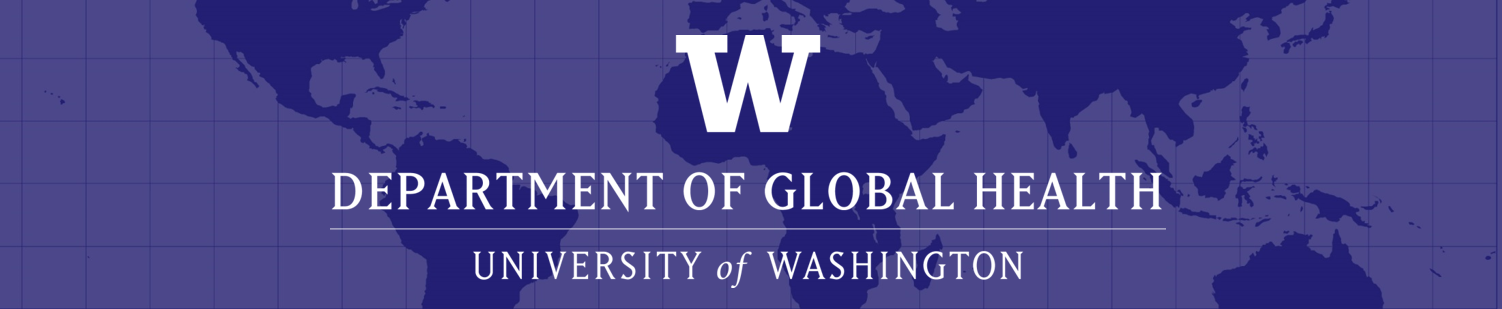
\includegraphics[width=21cm]{images/dgh_banner.png}};
 				\pgftext[x=1.1cm,y=24cm,bottom,left]{\fontsize{20}{20}{\textbf{\program}}};
 				\pgftext[x=1.1cm,y=23.2cm,bottom,left]{\fontsize{18}{18}{\textbf{\textcolor{grisfonce}\track}}};
 				\pgftext[x=10.5cm,y=16.5cm,bottom,center]{\fontsize{30}{30}{\textbf{Problems in HMIS \\ in Developing Countries}}};%\reporttitle
 				\pgftext[x=10.5cm,y=15.5cm,bottom,center]{\scalebox{0.77}[1]{\fontsize{20}{20}{\fontfamily{phv}\selectfont{}\textcolor{grisfonce}{\reportauthors}}}};
 				\pgftext[x=5.5cm,y=13.1cm,bottom,left]{\scalebox{0.6}[1]{\fontsize{18}{18}{\fontfamily{phv}\selectfont{}\textbf{\today}}}};
 				\pgftext[x=1.1cm,y=1.8cm,bottom,left]{
\includegraphics[width=6cm]{images/ihme_logo.png}};
                \pgftext[x=17cm,y=1.8cm,bottom,left]{
\includegraphics[width=3cm]{images/hai_logo.png}};
                \fill[fill=grisclair] (21cm,1cm) rectangle(0cm,0cm);
	\end{tikzpicture}
				};
			\end{tikzpicture}     
           
\end{titlepage}

%% Get the page after title empty
\pagenumbering{gobble}% Remove page numbers (and reset to 1)
\newpage\null\thispagestyle{empty}\newpage








%%%%%%%%%%%%%%%%%%%%%%%%%%%%%%%%%%%%%%%%%%%%%%%%%%%%%%%%%%%%%%%%%%
%%%%    	FRONT MATTER
%%%%%%%%%%%%%%%%%%%%%%%%%%%%%%%%%%%%%%%%%%%%%%%%%%%%%%%%%%%%%%%%%%
\thispagestyle{plain}
\pagenumbering{roman}
\setcounter{page}{1}



\paragraph{Abstract}

The way I approach HMIS design is through a common differentiation of four main functions : data collection, data management, data analysis and data use. My overall hypothesis is that current approaches to HMIS in sub-saharan Africa build systems that overly relying on data collection and underinvest in other functions, thus building systems that rely on frontline health workers, who have other roles to fill, while specialized personals at district and national levels are performing trivial operations. These systems are thus  mainly geared towards their reporting functions, neglecting patient care functions, and are by design inefficient for either of these functions. 

In my dissertation, I would like to explore tools and approaches that can correct the imbalance of these systems. I plan on working on 4 papers, one for each function of the HMIS :
\begin{enumerate}
\item	Data collection : I am working on an evaluation of the impact of the implementation of an EMR in HIV clinics in 341 hospitals in Kenya on the quality of care, and the ability of reporting to HIV program
\item	Data management : I am also currently working with the designers of OpenRBF to design a way to implement interoperability between OpenRBF and DHIS2. We have a designed a strategy for semantic interoperability between systems, and I will be testing this system in different settings and work on organizational interoperability.
\item	Data analysis : I plan on using HMIS data from different countries to test algorithms for facility performance monitoring based on reporting data.
\item	Data use : One of the reasons of the flow in current HMIS is for me the fact it is based on a function of administrative statistic thought as being justificative (workers presenting their results) and disciplinary (as a way to norm and supervise workers activity). This has been describe by Arjun Appadurai in the case of the production of statistics in colonial India, and is reinforced by an evolution of public statistics towards an evaluative value, as described by Alain Desrosières. I’d like to think on how these conditions of use of HMIS data are influencing the way the systems are thought and built, and how modifying this approach could help improve HMIS performances.
\end{enumerate}


% Table des matières
\cleardoublepage 
% Dans le cas du recto verso, ajoute une page blanche si besoin
\phantomsection
\tableofcontents
\addcontentsline{toc}{section}{Table of Content}
\newpage
\addcontentsline{toc}{section}{\listfigurename}
\listoffigures 
\newpage
\addcontentsline{toc}{section}{\listtablename}	
\listoftables

\thispagestyle{fancy}
	
% Justification moins stricte : des mots ne dépasseront pas des paragraphes
\sloppy
  
%%%%%%%%%%%%%%%%%%%%%%%%%%%%%%%%%%%%%%%%%%%%%%%%%%%
%%%% 	MAIN MATTER
%%%%%%%%%%%%%%%%%%%%%%%%%%%%%%%%%%%%%%%%%%%%%%%%%%%

%% Set page numbering right
\cleardoublepage
\pagenumbering{arabic} 
\setcounter{page}{1}

%% And Now get Writing !
\section{Introduction}

\subsection{Information in health systems}

The use of statistical information in the design, the implementation and the evaluation of public policies is of growing interest in different domain of public life. Different trends in the thoughts and traditions of public life have led to this strengthened importance. 

The improvement and the diffusion of tools and resources available for the production of public statistics have certainly be a first trend that has led to a better availability and use of data for decision making. In the meantime, the culture surrounding the production and use of numerical data in modern societies has evolved, both in reaction to increased capabilities of measurement, and of evolution of political and management sensibilities in these societies. 

The use of data for pubic decision is consubstantial to the apparition and the development of public as a domain of public action. The "invention of population" in the second half of the XVIIIth century was made possible by the reform and development of demographic information in Europe and the development of demographic methods. In later stages, the development of sampling and inferential statistics methods in the XIXth century was also key to the targeting of specific public health interventions. 

The use of data for policy making is thus, as we see, a combination of data sources, statistical methods, and political or social norms, that will define the conditions of utilisation of statistical evidence for policy making. Finding the proper data source, being able to analyze it and incorporating the results of this analysis in a political process is essential to the proper use and utilization of information systems.

In Global Health realm, the use of data for the definition of \textit{evidence based} intervention and policies has emerged as a panacea of project design and management. There are nonetheless difficulties in this regard. The global nature of public health means that statistical data available for analysis is by nature scattered and varied in nature, technical characteristics, quality and scope. In the meantime, the exigence of Global Health practitioners is to use and understand varied data sources in a unified global framework. The Global Burden of Disease initiative is a good example of this exigence of a global assessment of a wide variety of data from multiple contexts.

The challenge of using and processing different kinds of data varies with the nature of the data sources. The design and definition of survey data, for example, is governed by methodological and technical constraints that are comparable between settings and implementations. Meanwhile, data from health systems will be influenced by multiple factors, ranging from the administrative traditions in which they develop, to the level of resources involved in the design and building of these data systems, and to the type of activities performed in these systems. Among them, hospital data could arguably be considered the most impacted by these different factors.

\subsection{Importance of Health Management Information Systems}

Among different data sources Health Management Information Systems (HMIS) are specific in so far as they are designed and thought, from the very beginning, to fulfill multiple purposes. If a survey is implemented, the only objective of its data collection tools is to collect data fitted to the sole purpose of completing the survey's objectives. In the meantime, HMIS typically rely on personals and resources whose primary goal is not the collection of data, but have other functions in the health system. This is also a difference with data stemming from sources specialized systems, like a survey implementations, for which every resource involved is aiming at producing quality data.

This non specificity and non specialization of HMIS is key to understand both its importance and its challenges. The overarching importance of Health Management Information Systems (HMIS) in modern health systems\cite{foundph} is as well recognized as the inability of most developing countries to implement well-performing HMIS. HMIS are important to provide information on the BIBLIO.

The low performance of HMIS comes from multiple origins. BIBLIO.

We contend that the difficulty of designing and implementing HMIS that deliver usable information for decision makers comes from technical difficulties, as well as from detrimental technical and organizational choices. HMIS are primarily considered functions of a health systems, and not as primarily statistical systems. As a result, in many situations, the logics and choices that are made in health systems are guided by administrative culture and the organization of health care in specific contexts, and are not primarily designed to perform as data systems. In this regard, HMIS are mainly aimed at very specific goals, limiting interoperability of systems and building systems that are not flexbile and are not designed to give information outside of a very limited, preset framework.

M\&E = version la plus degradee

SUBSYSTEMS : cf document liberia

data coll : qu'est-ce qu'on apprend de metadonnees. comment peut aider comprehension du fonctionnement
data man : interoperability, data management
data analyse : quelle approche innovante ? qu'est-ce qu'on peut lire ?
politique : le role du statisticien public


\paragraph{what is and what is not part of HMIS} The reasons for this weakness are as varied as HMIS are complex objects. Many functions are involved in developing and implementing an HMIS. There are different views that can be adopted to describe a HMIS. Some authors privilegiate the demand side of HMIS, by describing HMIS trough their end users and why they need information. Some authors will privilegy goals of a specific HMIS users. Some authors will concentrate on describing what should be included as being part of an HMIS. Finally some other actors will prefer to address different functions that are exerted inside of HMIS. 

Even if the understanding of what should be considered part of a HMIS may vary depending on authors, every source regarding HMIS usually refers to the importance of using data for decision making at every level of health systems. 

In the meantime, there is a role for HMIS in organizing work in health systems more widely, as the way data is collected has an impact on how work is organized inside health systems. 

What are the main parts of HMIS ?

Different uses ?

Questions asked are at multiple levels.

Thinking about and working around HMIS requires different levels of thinking. 

organizational : what makes an HMIS work, and what functions should 
technological : right level of technology. adapt for best usage by different users (Illich)
analytical : what techniques of analysis to use with very specific data 
political : how this data should be used to inform decisions ?

The objective of this proposal is to shape our angle of analysis in each of these approaches, and to identify research directions that will help furthering the understanding of HMIS in developing countries and offer solutions for currently important issues.


DISCUTER LA SPECIFICITE DES HMIS EN PVD VS PAYS DEVELOPPES  => approche historique.

We adopt a statistican's approach to HMIS. 


\section{Two approaches to HMIS}

	\subsection{Functional approach}
	
A first way to approach HMIS is to describe the principal functions that are necessary to have a HMIS to run. Figure \ref{HMISFunctions} presents a simplified sketch of the principal functions that are to be filled in any HMIS. 

\begin{figure}[h]
\begin{center}
\begin{tikzpicture}[node distance=.8cm,  start chain=going below,]
     \node[punktchain, join] (DataCollection) {Data Collection};
     \node[punktchain, join] (DataManagement) {Data Transmission and Management};
     \node[punktchain, join] (DataAnalysis)   {Data Analysis};
     \node[punktchain, join] (DataUse) 		  {Data Use};
\end{tikzpicture}	    
\end{center}
\caption{Different functions inside the Health Information Systems}
\label{HMISFunctions}
\end{figure}           

Four main functions can be found in HMIS. 

\paragraph{Data Collection} Primary data collection is essential to the production of any information system. In the case of HMIS, data collection happens in health facilities, and is made by health professionals.

Data collected in facilities can be individual patient data collected in patients files or cards. It can also be a first level of aggregation of this data, as for indicators that are reported on a regular basis by facilities to higher levels of the health system. This reporting usually happen through standardized reports, and are then transmitted by successive aggregation to the top of the health pyramid.

\paragraph{Data Management} Data collected in health facilities has to be stored and archived, to be later accessed and reused. Data management work can encompass managing paper data, or managing computerized data. Individual patient data will be computerized in Electronic Medical Records (EMR) whereas aggregated indicators are stored in data-warehouses, of the type of the DHIS2 software.

\paragraph{Data Analysis} Data that is collected and stored in HMIS can then be analyzed. The type of analysis that is doable with EMR data will be different from the type of analysis that is possible to make with indicator type data. 

\paragraph{Data Usage} What kind of decisions ? Memoire Cheickna.


	\subsection{Goal approach}

Another approach to HMIS is a consideration of the stated goals of these information systems. Figure \ref{HMISGoals} shows what these goals are. The pyramidal representation of these needs is used to show that these goals fill data needs at different levels of health systems.

\begin{figure}[htp]
\centering
\begin{tikzpicture}[node distance=2cm]
\coordinate (A) at (-4.5,0) {};
\coordinate (B) at ( 4.5,0) {};
\coordinate (C) at ( 0,7.7942) {};
\draw[name path=AC] (A) -- (C);
\draw[name path=BC] (B) -- (C);
\draw (1.1,5.8971)--(3.5,5.8971) ;
\draw(3.5,5.8971)--(3.5,3) ;
\draw [->](3.5,3)--(2.77,3) ;
\node at (4.4,4.25) {Feedback};
\foreach \y/\A/\txtHigh in {0/Patients Care/0.8 ,2/Facility Administration \\ and Reporting/2.5,4/Planning \\ Monitoring \\ \& Evaluation /4.8}{
    \path[name path=horiz] (A|-0,\y) -- (B|-0,\y);
    \draw[name intersections={of=AC and horiz,by=P},
          name intersections={of=BC and horiz,by=Q}] (P) -- (Q)
          node[align = center,above] at (0,\txtHigh){\A};
          }         
\end{tikzpicture}
\caption{Objectives of HMIS}
\label{HMISGoals}
\end{figure}

\paragraph{Patients Care} Taking care of patients is the primary goal of a health facility. To do so, it is necessary to collect data on these patient, data that will be transmitted (to other services), stored and reused during further follow-ups. 

\paragraph{Facility Administration and Reporting} At facility level, HMIS data is used in daily activities to quantify and forecast needs in health inputs, and to create reports for higher levels of the health system. 

\paragraph{Planning, Monitoring \& Evaluation } People in charge of the administration of health systems at local or national also need data to monitor activities in the health system, to evaluate the results of interventions, to report to funders or to plan later interventions.

	\subsection{Political analysis}

A last approach to HMIS is to take a political approach to their needs. Information systems are as numerical and scientific systems, are often considered as being non political. Reflexion on HMIS then concentrates on the functions and goals and HMIS and articulates the formers with the later. Meanwhile, this is hardly a sufficient approach to it. HMIS, as they compose health systems, are political objects. The way they evolve is driven by assumptions, ... We posit that if the goals we have displayed earlier are the ones that are considered the most important for HMIS, they may not be the most important when we consider how HMIS are being implemented.

\subsubsection{Interdependence of functions}

In tackling a technical system, we need to keep in mind its technical aspects as well as its human aspects.

This functions are interdependent with each other. Data collection is key to enable other functions. Absence of data means there is nothing to be managed, nor to be analyzed or used. This importance of the availability of data has been recognized and is key to intervention to improve the quality of data collected in developing countries health systems. Meanwhile, we argue the focus on the collection function of HMIS may be to important and can be counter productive.

Most of interventions to improve HMIS are geared toward improving \textit{data quality} or its availability, all characteristics that concern the data collection function. Meanwhile, facility reporting 

Problème est l'équilibrage des différentes fonctions. Mauvaise articulation. Comment rééquilibrer.

Statistique publique

Non adptation de l'administration et des systèmes utilisés, comme montré dans le cas de l'algérie

Data collection should be the same for all the goals. Highly specialized data collection. Low specialization of other functions. This shows a bizarre profile. Data users everywhere. Very little data specialists.


\subsubsection{Data collection as entry point}
Le patient comme objectif de la collecte des données

Un data management important

Analyse

Réévaluation de la causalité. On veut améliorer ce qui se passe dans les niveaux supérieurs  pour améliorer le fonctionnement de la collecte des donnée. 

Comment faire pour améliorer l'utilisation des données dans les systèmes de santé. Quels sont les aspects importants ?

Theory of change for HMIS ?

\subsubsection{The legacy of colonial statistics}

Question de la statistique coloniale. Les différents niveaux de la statistique administrative, importance de la justification et du contrôle dans l'utilisation faites des données administratives.

There is a primary problem in the use of HMIS data. Alain Desrosières has shown the richness and complication of the production and use of statistics in modern societies. Desrosières shows how two traditions have been cohabiting in the early ages of the production of social statistics\cite{admin_savant}. 

\begin{quote}
"The first tradition is administrative, and is based on political science and the law, on the German Staatenkunde, from the time of Conring and Achenwall. It is more taxonomic than metrological: it is designed to classify facts systematically rather than measure them, which is the essence of the other tradition, the "English" tradition. The latter, inspired more by the natural sciences and by progress made in measurement and probability theories, is a distant relation of the English political arithmetic of Graunt and Petty."
\end{quote}

Desrosières later shows how these two traditions have bee reconciled in the modern figure of the statistician, at the same time administrator and scientist. It is useful to keep considering this tension when thinking about maturing statistical systems like developing countries' HMIS. Being able to distinguish between situations when actors of HMIS are acting as administrators, and when the position is that of a metrician is essential to understand HMIS issues and offer informed solutions. 

This distinction is essential at many levels. The whole debate around the level of uncertainty that is bearable around a measurement is not only important for statisticians. Choosing a given approach will have an impact on how primary data will be collected, how it will be analyzed, and how it will be used. In many usages of HMIS, complete enumeration is deemed necessary, but this can be discussed. What is the level of confidence one can bear around the estimation of a stock of drugs ?

In other dimensions, how can civil society help for HMIS design and evaluation


\section{Problems with HMIS}

	\subsection{Care improvement}
	
	\begin{figure}[htp]
\begin{minipage}{.4\textwidth}
\begin{tikzpicture}[node distance=.8cm,  start chain=going below,]
     \node[punktchain, join] (DataCollection) {Data Collection};
     \node[punktchain, join] (DataManagement) {Data Transmission and Management};
     \node[punktchain, join] (DataAnalysis)   {Data Analysis};
     \node[punktchain, join] (DataUse) 		  {Data Use};
     \filldraw[ultra thick, draw=black, fill=green, opacity=0.2] (-2.2,-.7) -- (-2.2,.7) -- (2.2,.7) -- (2.2,-.7) -- (-2.2,-.7) ;
\end{tikzpicture}	
\end{minipage}
\begin{minipage}{.5\textwidth}
\begin{tikzpicture}[node distance=2cm]
\coordinate (A) at (-4.5,0) {};
\coordinate (B) at ( 4.5,0) {};
\coordinate (C) at ( 0,7.7942) {};
\draw[name path=AC] (A) -- (C);
\draw[name path=BC] (B) -- (C);
\draw (1.1,5.8971)--(3.5,5.8971) ;
\draw(3.5,5.8971)--(3.5,3) ;
\draw [->](3.5,3)--(2.77,3) ;
\node at (4.4,4.25) {Feedback};
\foreach \y/\A/\txtHigh in {0/Patients Care/0.8 ,2/Facility Administration \\ and Reporting/2.5,4/Planning \\ Monitoring \\ \& Evaluation /4.8}{
    \path[name path=horiz] (A|-0,\y) -- (B|-0,\y);
    \draw[name intersections={of=AC and horiz,by=P},
          name intersections={of=BC and horiz,by=Q}] (P) -- (Q)
          node[align = center,above] at (0,\txtHigh){\A};
          }         
    \filldraw[ultra thick, draw=black, fill=green, opacity=0.2] (-4.7,-.2) -- (-4.7,2.2) -- (4.7,2.2) -- (4.7,-.2) -- (-4.7,-.2) ;
\end{tikzpicture}
\caption{Objectives of HMIS}

\end{minipage}
\label{Paper One}
\end{figure}

A first question we want to ask 

	\subsection{Interoperability}


\begin{figure}[ht]
\begin{center}
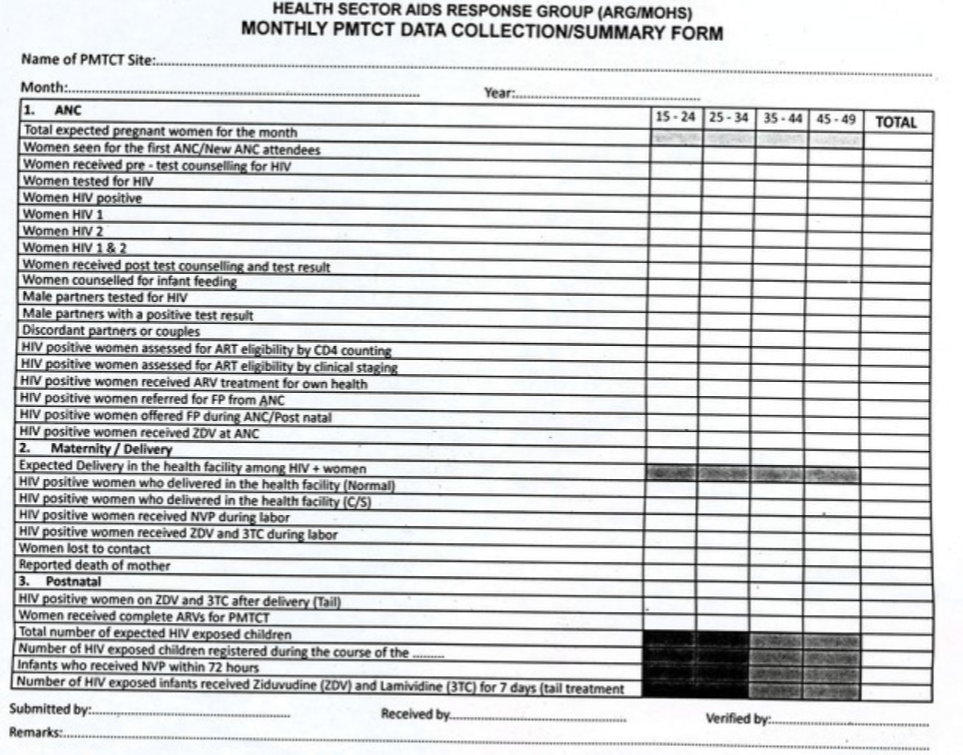
\includegraphics[scale=0.5]{figure/Picture1.png} 
\caption{Figure Test}
\end{center}
\end{figure}


		\subsection{Data analysis with bad data quality}  

\begin{table}[ht]
\begin{tabular}{cccc}
\hline 
 					& Individual Health & Local Management & Program Management \\ 
\hline 
Computerization & & \\
\hline
Interoperability 	& Sharing data between applications  &  &  \\ 
\hline 
Data Analysis &  &  &  \\ 
\hline 
\end{tabular} 
\caption{Matrix of HMIS problematics}
\end{table}

TABLE : Intersection of the two types of problems
	
	\subsection{Pending questions}

Ici on selectionne les questions a regarder et eclairer dans le cadre de la these.

\section{Planned papers}

We are planning to write and publish 3 papers that will each allow us to get an insight in 3 important aspects of our 

	\subsection{EMR and individual health}

Data from ITech

	\subsection{Interoperability }
 
Follow-up on a project with Bluesquare  / try grouping indicators based on actual series
 
	\subsection{Analysis}  
  
Evaluation of facility performance / screening / prediction of quality

	\subsection{Data Use}
  
Reflections on social conditions of HMIS data usage  / politics of administrative statistics.

Data is not produced to create knowledge, but to implement disciplinary monitoring. Thinking mainly in terms of indicators. 

Case study : analyse de textes M\&E / projets de reforme de systemes hmis, et analyse de la vision des HMIS qu'ils proposent. quelle place pour la societe civile ? inversion des priorites. 
  
%%%%%%%%%%%%%%%%%%%%%%%%%%%%%%%%%%%%%%%%%%%%%%%%%%%
%% 			BIBLIOGRAPHY
%%%%%%%%%%%%%%%%%%%%%%%%%%%%%%%%%%%%%%%%%%%%%%%%%%%
%\cleardoublepage
%\phantomsection\addcontentsline{toc}{section}{Références}
\newpage
\bibliography{bibliographie}


\end{document}

